  This section prensent the test results.

  Firstly I  present the performance difference between TCP and UDP used as the OpenVPN protocol by testing the throughput and the number of request/response per second.
  Secondly I test the behavior of MPTCP using link with different RTT and bandwith.
  Finally I try different congestion control and analyse wether it help increasing performances.

 \section{TCP vs UDP}

  In this section I compare the througput of a TCP connection using TCP and UDP as the OpenVPN tunnel protocol to determine where MPTCP can be interesting and where not.
  Many combinaison of bandwidth and delay will be used they will be specified for each test.
  The size of the openvpn buffers will also be specify as it plays a role in the overall throughput.
  TCP windows autotuning mechanism of Linux will always be enable.

  \subsection{Bulk data transfer} \label{sec:bulk_data_transfer}

  This first test is a bulk data transfer.

  Test setup :

  \begin{itemize}
  \item First link bandwith of 8mbit/s, 32mbit/s, 100mbit/s  and RTT: 2ms (default route)
  \item Second link bandwith of 8mbit/s, 32mbit/s, 100mbit/s  and RTT: 2ms
  \item Using default mptcp scheduler
  \item OpenVPN buffer default size 65536 bytes on client and server
  \item Congestion control : cubic
  \end{itemize}

  \begin{figure}[h!]
    \centering
    \includegraphics[width=14cm]{../results/tcp_vs_udp_2ms.pdf}
    \caption{TCP vs UDP RTT: 2ms Buffer size: 64k}
    \label{all_tcp_vs_udp}
  \end{figure}

  When using TCP as the OpenVPN protocol, MPTCP will creates two subflows, one on each link. Actually the full-mesh path manager create four subflow on this setup
  but the cross IP subflows has been blocked with the help of IPTables rules. On the other hand UDP will only use one of the available links.

  For this test my hypothesis is that using MPTCP would always give a better throughput because it can use double of the bandwith than UDP can.

  However results in figure \ref{all_tcp_vs_udp} shows that TCP is faster than UDP for small maximum bandwidth like 8 or 32mbit/s but for greater maximum bandwidth like 100mbit/s,
  TCP is slower than UDP.

  Besides, for the 32mbit/s bandwidth, the capacity of the two links are not fully used otherwise the throughput would be of about 60-64mbit/s.
  Further, even when using UDP and a maximum of 100mbit/s bandwidth, the whole bandwidth available is not used.

  These results are mainly due to two things :
  \begin{enumerate}
    \item The router CPU is used at about 100\% while the tests are running for the 32mbit/s (tcp) and 100mbit/s (tcp and udp) maximum link bandwidth
    \item TCP over TCP can be bad because it can trigger multiple retransmissions \cite{tcpovertcp}
  \end{enumerate}

The first reason is linked to the fact that the router has to encapsulate and decapsulate the packet from the OpenVPN tunnel as explained in section \ref{sec:section_openvpn}
causing the router to switch between kernel space and
userspace. This is very costly in CPU cycle and the router CPU is a bit too weak.

The second reason relates to having two layers of TCP connection.
TCP is a protocol that assumes an unreliable carrier. So if you have multiple layers of TCP connections each layer will guarantee that every data arrive to the other end.
If the encapsulating or Internet layer drops a packet, both TCP streams will attempt to correct the error and retransmit duplicate data.
This queues up data transmissions exponentially and slow down the data transmission.

Bofre concluding, it is interesting to analyse how the traffic was split accross the subflows. For this, I used \textit{tcpdump} to capture packets and \textit{mptcptrace} to analyse these captures.
The traffic was captured on the OpenVPN server, on the sending side, to avoid having too much stress put on the router.

The sequence graphic generated by mptcptrace showed that the traffic was well splitted accross the subflows, which is the expected result because the scheduler used during these tests was the default and both links had the same RTT and same bandwidth.

Figure \ref{mptcptrace_subflow} showshow the traffic was split. When the green line approaches the $+1$ limit,
it is the initial subflow which is mainly use and when the blue line approaches the $-1$ limit it is the second subflow which is mainly use.
Here, the two lines are near 0, meaning that they are both used equaly.

  \begin{figure}[h!]
    \centering
    \includegraphics[width=16cm]{../results/subflow_split.pdf}
    \caption{MPTCP Subflows Balance}
    \label{mptcptrace_subflow}
  \end{figure}

  To conclude for this test, even if UDP is faster than TCP in some cases, it should bet taken into account that with UDP if the link fails, the connection is lost.
  Depending on what you are looking for, it can be usefull to have a more robust connection even if it is slower and in that case use TCP.


   \subsection{Delay introduced on links} \label{sec:delay_on_links}

   This section presents the same test than in section \ref{sec:bulk_data_transfer} adding the insertion of delay on links and I then analyse which effect it has on the throughput. The delay are 25ms and 200ms on both links which give a 50RTT and a 400RTT. The buffers sizes are the default OpenVPN buffer size, 64k.

On figure \ref{tcp_vs_udp_200ms} the effect of delay on the througput using TCP and UDP as OpenVPN protocol is presented

\begin{itemize}
\item For TCP the OpenVPN buffer size (64k) is a real disaster and the overall speed is very low compared to the 2ms RTT (see figure \ref{all_tcp_vs_udp}).
\item For UDP he OpenVPN buffer size is not as bad as for TCP but the overall speed still decrease a lot.
\end{itemize}

For TCP this is mainly caused by wrong buffer size. Indeed the computation of the maximum throughput possible with a buffer of 64k and a RTT of 400ms
is obtain 1.3Mbit/s. The same computation for a RTT of 50ms is 10Mbit/s. This is show on figure \ref{tcp_vs_udp_200ms}.

Figure \ref{window_tcp_32_50_full} is the windows graph created by mptcp for the link bandwith of 32mbit/s with a RTT of 400ms. You can see that the window is totally full.

\begin{figure}[h!]
 \centering
 \includegraphics[width=1\textwidth]{../results/all_tcp_vs_udp_200ms.pdf}
 \caption{TCP vs UDP with high RTT buffer: 64k}
 \label{tcp_vs_udp_200ms}
\end{figure}

\begin{figure}[h!]
 \centering
 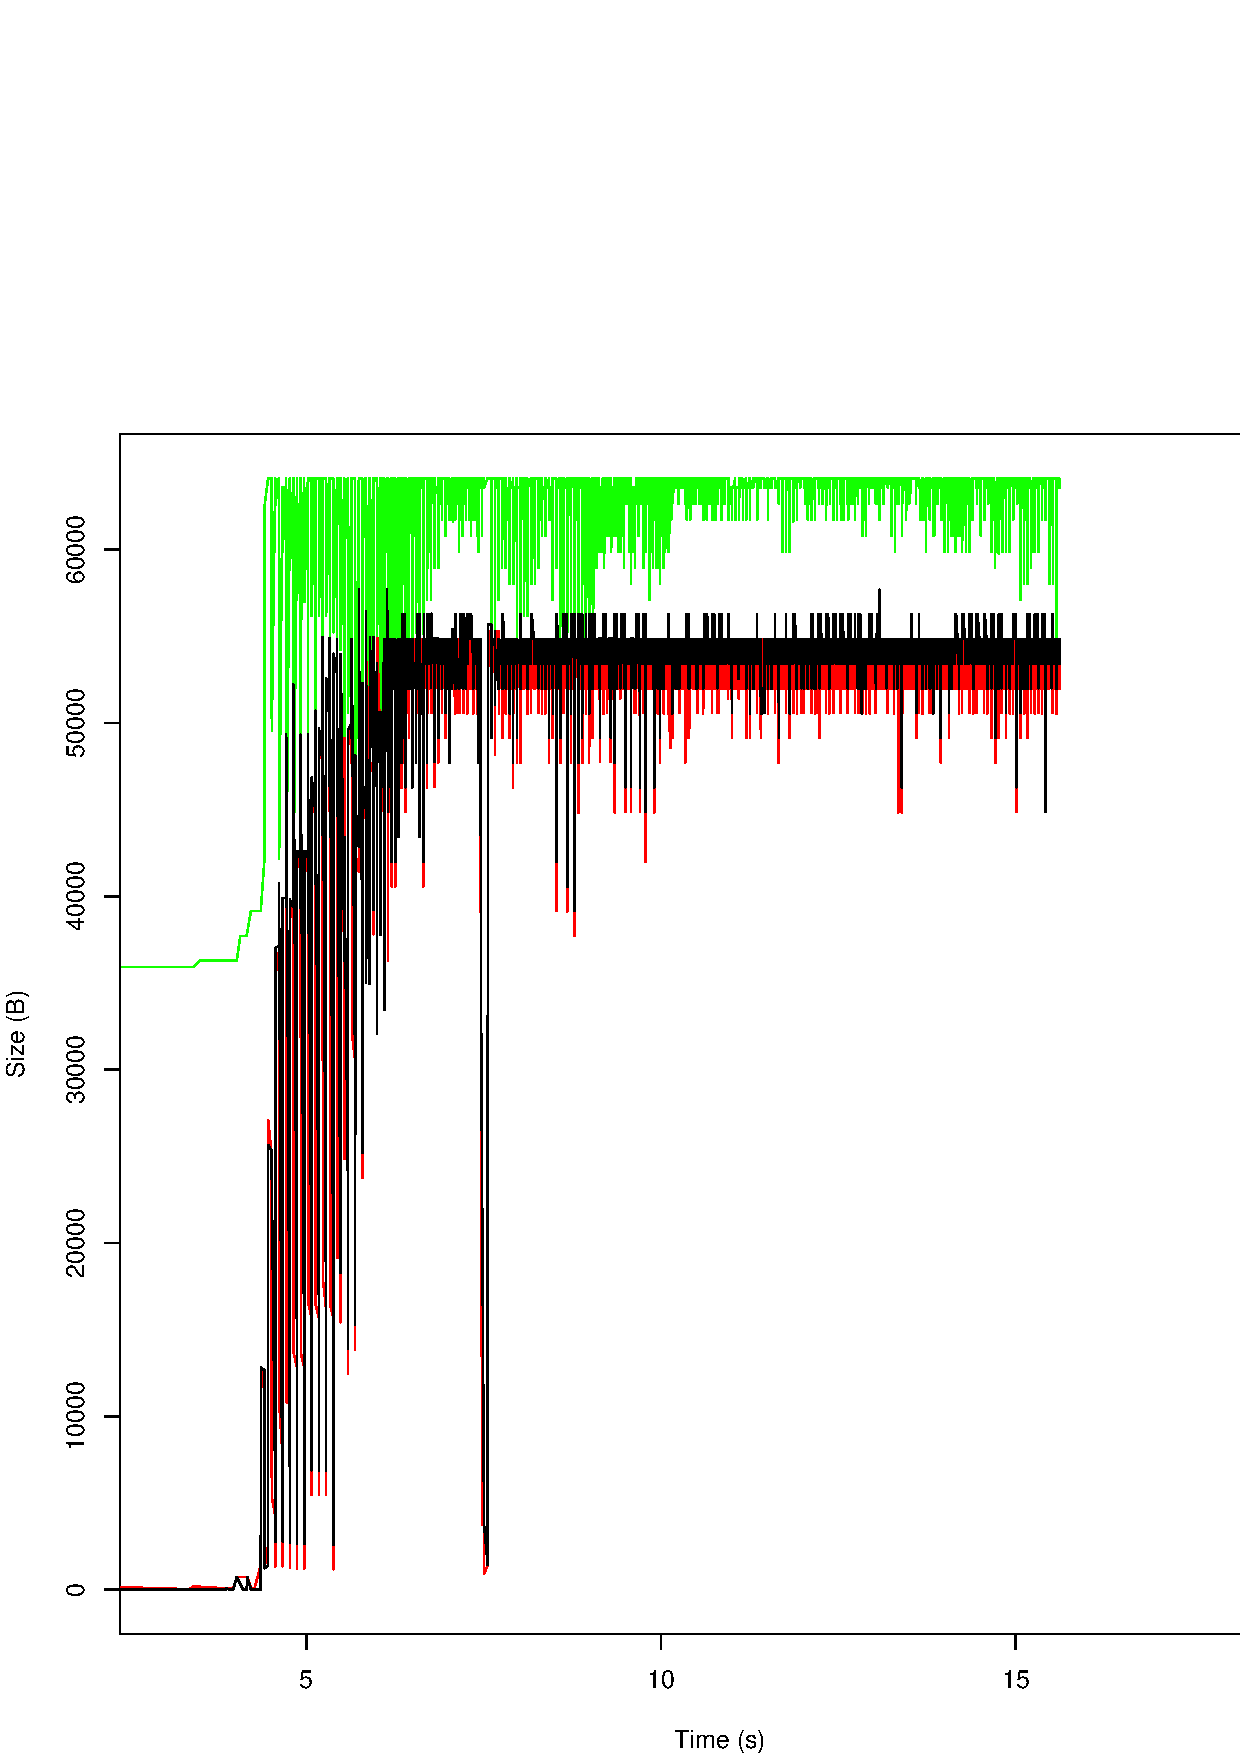
\includegraphics[width=10cm]{../results/window_tcp_32_50_full.pdf}
 \caption{TCP Window being full}
 \label{window_tcp_32_50_full}
\end{figure}

This time the router CPU is around 20\%-30\% usage so there is no bottleneck.
Section \ref{sec:improving_throughput} presents and attempt to resolve this situation by changing buffer size on the openvpn client and openvpn server.

\newpage

\subsection{Request/Response}

In this section I test the number of request / response per second when using TCP or UDP as the OpenVPN protocol. In this purpose I use test from Netperf and Apache Benchmark tool.
My goal is to determine wether a browsing experience for a user would be possible or not depending on the network.

\subsubsection{TCP\_CRR}

  Test setup :

  \begin{itemize}
  \item First link bandwith of 8mbit/s, 32mbit/s, 100mbit/s  and RTT: 2ms, 400ms (default route)
  \item Second link bandwith of 8mbit/s, 32mbit/s, 100mbit/s  and RTT: 2ms, 400ms
  \item Using default mptcp scheduler
  \item OpenVPN buffer default size 65536 bytes on client and server
  \item Congestion control : cubic
  \item Request message size : 1 byte
  \item Response message size : 1 byte
  \end{itemize}

  \begin{figure}[h!]
    \centering
    \includegraphics[width=16cm]{../results/tcp_vs_udp_transaction.pdf}
    \caption{TCP vs UDP transaction per second request and response size : 1 byte}
    \label{tcp_vs_udp_transaction}
  \end{figure}

  In this test the CPU and links bandwith do not seems to be the bottleneck. What seems to be the problem is the overhead due to creating and destroying TCP connection for each transaction.

  Figure \ref{tcp_vs_udp_transaction} shows that UDP seems to be a bit better. TCP being a connection-oriented protocol, it takes a bit more time to set up a connection than UDP.
  On top of that, the amount of data to be transmitted inside one transaction is very small, which means that a single connection is destroyed almost immediatly and it creates another one right away,
  this make the connection setup time very impactful.

  In figure \ref{tcp_vs_udp_transaction} is also visible the huge effect of the delay on the number of transaction per second,
  goes up to 400 transaction per second with a RTT of 2ms and it goes down to 2 transaction per second with a RTT of 400ms.

  A high RTT, means that the creation and the teardown of a connection takes more time and because the test are synchronous,
  A transaction has to wait for the previous one transaction to finish before starting.

  Increasing the data transmited into one transaction would be a more realistic and fair test between TCP and UDP.
  I used a 100 bytes request message size and a 170 bytes response message size to have identical size than the test done with Apache Benchmark (see section \ref{sec:ab}).

  \begin{figure}[h!]
    \centering
    \includegraphics[width=16cm]{../results/tcp_vs_udp_transaction_fair.pdf}
    \caption{TCP vs UDP transaction per second request size : 100 / response size : 170 byte}
    \label{tcp_vs_udp_transaction_fair}
  \end{figure}

  Figure \ref{tcp_vs_udp_transaction_fair} shows that the difference between TCP and UDP is smaller because the data transmitted inside one transaction is bigger and
  the connection setup time has less impact. However the effect of the delay is still very strong and confirm my previous conclusion.

  In conclusion, for this kind of traffic, MPTCP will not improve performance. The advantage of using multiple paths is not very usefull (only if one path fails) because it has no concurrent transaction
  and they are executed synchronously. In this case, UDP seems to be a better choice.

  Hewever these tests might not reflect reality because normaly one would use one TCP connection for multiple transactions
  and  establish multiple connections, unfortunatly Netperf does not provide such a test. To do that I use Apache Benchmark see section \ref{sec:ab} below.

\subsubsection{Apache Benchmark (AB)} \label{sec:ab}

The choice to run AB is to provide a more realistic way to test the process of request\/response to a real web server.
It also gives the possibility to use simultanious connections with the http \textit{keep-alive} option.

When \textit{keep-alive} option is set to true, it uses a single TCP connection to send and receive multiple HTTP request/response,
as opposed to opening a new connection for every single request/response transaction like in TCP\_CCR from netperf.

The settings used to run AB are :

\begin{itemize}
\item 6 concurrent connections, usually browser use between 6(Firefox,Chrome) and 8(Opera)
\item maximum time of 60 seconds
\item option \textit{keep-alive} enable
\end{itemize}

AB always stops after 50000 transaction even if the total time has not been totaly spent.
The requests made by AB have a size of 100 bytes and the responses by the Apache server have a size of 170 bytes.

   \begin{figure}[h!]
    \centering
    \includegraphics[width=1\textwidth]{../results/all_request_response_ab.pdf}
    \caption{Request/Response Apache benchmark}
    \label{all_request_response_ab}
  \end{figure}

Figure \ref{all_request_response_ab} shows that the number of transactions with UDP and TCP using apache benchmark. The number are quite bigger than the one from the previous tests TCP\_CRR.
The maximum is 1800 transactions per second when using UDP and a RTT of 2ms. The minimum is 6 transactions per second when using TCP and having a RTT of 400ms.

The links maximum bandwith do not have a big impact on the number of transaction per second, it is
mainly the RTT. In this test UDP still dominate even with the concurrent connections being used.

It is the same as the TCP\_CRR test: the CPU and link bandwith are not the bottle neck,
the CPU usage of the router is around 25-30\% during the tests. The problem is the time it takes to establish a connection when using TCP.

In conclusion, TCP gives reasonnable performances compared to UDP and This leads me to think that it could be used without impacting too much on the user experience.

New, I look at what happen if the main link fails during a certain span of time to evaluate wether in this case MPTCP has the advantage.

The test length is 30 second and the main link will be set to 100\% packet loss after 5 seconds and then set back to 0\% after 15 seconds.
The links RTT are 2ms and max bandwidth is 8mbit/s and 32mbit/s.

On figure \ref{request_response_link_down_ab}, we see that this time the difference between the transaction per second for UDP and TCP is smaller because TCP continue to transmit data while
UDP is stopped.

Inserting more down time on the link makes this behavior even more visible and UDP is slower than TCP.
This is because MPTCP switches the traffic to another subflow when it finds out that the one it is using starts to have timeout.
UDP however cannot do that and will not be able to transmit data during this time.

   \begin{figure}[h!]
    \centering
    \includegraphics[width=8cm]{../results/request_response_link_down_ab.pdf}
    \caption{Request/Response Apache benchmark one link down}
    \label{request_response_link_down_ab}
  \end{figure}

   \begin{figure}[h!]
    \centering
    \includegraphics[width=8cm]{../results/request_response_subflow_change.pdf}
    \caption{Request/Response Apache benchmark one link down subflow details}
    \label{request_response_subflow_change}
  \end{figure}


Figure \ref{request_response_subflow_change} is the sequence number graph of the MPTCP connection.
It presents the switch from the main subflow (the green line) to the alternative subflow (the blue line) when the link goes down.

\section{Links with different bandwidth and delay}

For these tests I go back to builk data transfer test and I look at the impact on the throughput when using links with different bandwith and delay.
Here I only use TCP has OpenVPN protocol. UDP is not very interesting because it only uses one link.

This is interesting because we will see how MPTCP decides to split traffic on the two subflows depending on their RTT and their bandwidth.

\subsection{First test setup} \label{sec:first_test}

\begin{itemize}
\item First link bandwith of 32mbit/s and RTT: 2ms (default route)
\item Second link bandwith of 8mbit/s and a RTT: 2ms
\item Using default mptcp scheduler
\item OpenVPN buffer set to 64000 byte (TCP windows size) on client and server
\item Congestion control : cubic
\end{itemize}

In theory we would like to get around 40mbit/s of throughput. In practice we get a 35mbit/s througput, the router is not the bottleneck the CPU is utilized around 60\%.

This setup will be used for further tests in section \ref{sec:improving_throughput_congestion_control}

\subsection{Second test setup}

\begin{itemize}
\item First link bandwith of 32mbit/s and RTT: 2ms (default route)
\item Second link bandwith of 8mbit/s and a RTT: 400ms
\item Using default MPTCP scheduler
\item OpenVPN buffer set to 400000 byte (TCP windows size) on client and server
\item Congestion control : cubic
\end{itemize}

In theory we would expect a throughput around 40mbit/s which is the sum of the two link Bandwith.

In practice MPTCP only uses the link with the lowest RTT and does not use the second link, this gives a throughput around 30mbit/s.

To analyse how the traffic splits accross the two subflows I use MPTCPtrace to generate the sequence number graph and a script provided by Benjamin Hesmans to generate figure \ref{32_8-2_400rtt_seq}.
On this figure the balance is close to the +1 limit meaning that the traffic is mainly on first subflow (first link) and the second subflow (second link) is rarely used.

The analyse of the sequence graph (not presented) shows that because of the high RTT on the second subflow, packets send on this subflow, are reinjected on the first subflow.

\begin{figure}[h!]
 \centering
 \includegraphics[width=14cm]{../results/32_8-2_400rtt_seq2.pdf}
 \caption{Subflow usage graph second test setup}
 \label{32_8-2_400rtt_seq}
\end{figure}

\subsection{Third test setup} \label{sec:third_test}

\begin{itemize}
\item First link bandwith of 32mbit/s and RTT: 400ms (default route)
\item Second link bandwith of 8mbit/s and RTT: 2ms
\item Using default MPTCP scheduler
\item OpenVPN buffer set to 1600000 byte (TCP windows size) on client and server
\item Congestion control : cubic
\end{itemize}

\begin{figure}[h!]
 \centering
 \includegraphics[width=14cm]{../results/32_8-400_2rtt_seq2.pdf}
 \caption{Subflow usage graph third test setup}
 \label{32_8-400_2rtt_seq}
\end{figure}

Here MPTCP use both links but the throughput is only around 8mbit/s. Figure \ref{32_8-400_2rtt_seq} shows that it uses the second subflow (second link) in blue and
 also the first subflow (first link) quite often.

If we look at the sequence graph (not presented) we see that it retransmit some packet from the first subflow to the second subflow because of the high RTT of the first subflow.

In conclusion for some of these setups MPTCP are not optimal and there is room for improvement.
In section \ref{sec:improving_throughput_congestion_control} and \ref{sec:improving_throughput_scheduler}
I will use differents congestion control algorithms and a alternative MPTCP scheduler and check wether it is more adequate.
